% Options for packages loaded elsewhere
% Options for packages loaded elsewhere
\PassOptionsToPackage{unicode}{hyperref}
\PassOptionsToPackage{hyphens}{url}
%
\documentclass[
  indonesian,
  letterpaper,
]{scrbook}
\usepackage{xcolor}
\usepackage[paperwidth=8.27in, paperheight=11.69in, top=0.8in,
bottom=1in, left=1in, right=1in]{geometry}
\usepackage{amsmath,amssymb}
\setcounter{secnumdepth}{5}
\usepackage{iftex}
\ifPDFTeX
  \usepackage[T1]{fontenc}
  \usepackage[utf8]{inputenc}
  \usepackage{textcomp} % provide euro and other symbols
\else % if luatex or xetex
  \usepackage{unicode-math} % this also loads fontspec
  \defaultfontfeatures{Scale=MatchLowercase}
  \defaultfontfeatures[\rmfamily]{Ligatures=TeX,Scale=1}
\fi
\usepackage{lmodern}
\ifPDFTeX\else
  % xetex/luatex font selection
\fi
% Use upquote if available, for straight quotes in verbatim environments
\IfFileExists{upquote.sty}{\usepackage{upquote}}{}
\IfFileExists{microtype.sty}{% use microtype if available
  \usepackage[]{microtype}
  \UseMicrotypeSet[protrusion]{basicmath} % disable protrusion for tt fonts
}{}
\makeatletter
\@ifundefined{KOMAClassName}{% if non-KOMA class
  \IfFileExists{parskip.sty}{%
    \usepackage{parskip}
  }{% else
    \setlength{\parindent}{0pt}
    \setlength{\parskip}{6pt plus 2pt minus 1pt}}
}{% if KOMA class
  \KOMAoptions{parskip=half}}
\makeatother
% Make \paragraph and \subparagraph free-standing
\makeatletter
\ifx\paragraph\undefined\else
  \let\oldparagraph\paragraph
  \renewcommand{\paragraph}{
    \@ifstar
      \xxxParagraphStar
      \xxxParagraphNoStar
  }
  \newcommand{\xxxParagraphStar}[1]{\oldparagraph*{#1}\mbox{}}
  \newcommand{\xxxParagraphNoStar}[1]{\oldparagraph{#1}\mbox{}}
\fi
\ifx\subparagraph\undefined\else
  \let\oldsubparagraph\subparagraph
  \renewcommand{\subparagraph}{
    \@ifstar
      \xxxSubParagraphStar
      \xxxSubParagraphNoStar
  }
  \newcommand{\xxxSubParagraphStar}[1]{\oldsubparagraph*{#1}\mbox{}}
  \newcommand{\xxxSubParagraphNoStar}[1]{\oldsubparagraph{#1}\mbox{}}
\fi
\makeatother


\usepackage{longtable,booktabs,array}
\usepackage{calc} % for calculating minipage widths
% Correct order of tables after \paragraph or \subparagraph
\usepackage{etoolbox}
\makeatletter
\patchcmd\longtable{\par}{\if@noskipsec\mbox{}\fi\par}{}{}
\makeatother
% Allow footnotes in longtable head/foot
\IfFileExists{footnotehyper.sty}{\usepackage{footnotehyper}}{\usepackage{footnote}}
\makesavenoteenv{longtable}
\usepackage{graphicx}
\makeatletter
\newsavebox\pandoc@box
\newcommand*\pandocbounded[1]{% scales image to fit in text height/width
  \sbox\pandoc@box{#1}%
  \Gscale@div\@tempa{\textheight}{\dimexpr\ht\pandoc@box+\dp\pandoc@box\relax}%
  \Gscale@div\@tempb{\linewidth}{\wd\pandoc@box}%
  \ifdim\@tempb\p@<\@tempa\p@\let\@tempa\@tempb\fi% select the smaller of both
  \ifdim\@tempa\p@<\p@\scalebox{\@tempa}{\usebox\pandoc@box}%
  \else\usebox{\pandoc@box}%
  \fi%
}
% Set default figure placement to htbp
\def\fps@figure{htbp}
\makeatother



\ifLuaTeX
\usepackage[bidi=basic,provide=*]{babel}
\else
\usepackage[bidi=default,provide=*]{babel}
\fi
% get rid of language-specific shorthands (see #6817):
\let\LanguageShortHands\languageshorthands
\def\languageshorthands#1{}


\setlength{\emergencystretch}{3em} % prevent overfull lines

\providecommand{\tightlist}{%
  \setlength{\itemsep}{0pt}\setlength{\parskip}{0pt}}



 


% Warna judul agar mirip contoh (beige keemasan halus)
\usepackage{xcolor}
\definecolor{titleaccent}{RGB}{183,176,138} % #b7b08a

% Paket yang diperlukan
\usepackage{pdfpages}   % untuk menyisipkan cover.pdf
\usepackage{graphicx}   % untuk cover berbentuk gambar (opsional)

% Nonaktifkan title bawaan Pandoc (\maketitle) agar tidak dobel
\makeatletter
\AtBeginDocument{\let\maketitle\relax}
\makeatother

% --- Pastikan judul bab & isi berada di halaman yang sama (KOMA-Script) ---
%\KOMAoptions{titlepage=false,open=any} % redundan dengan YAML, tapi aman dipaksa di runtime

% Pangkas jeda atas/bawah judul bab agar tidak “lompat” ke halaman berikut
%\RedeclareSectionCommand[
 % beforeskip=-1.2\baselineskip, % negatif = teks langsung menyusul di halaman yang sama
  %afterskip=.8\baselineskip,
  %afterindent=false
%]{chapter}

\usepackage{afterpage}
\graphicspath{{images/}} 

\usepackage{fontspec}
\setmainfont{Georgia}
\setsansfont{Georgia}
\setmonofont{Courier New} % monospaced font alternatif, karena Georgia tidak punya varian mono
\makeatletter
\@ifpackageloaded{bookmark}{}{\usepackage{bookmark}}
\makeatother
\makeatletter
\@ifpackageloaded{caption}{}{\usepackage{caption}}
\AtBeginDocument{%
\ifdefined\contentsname
  \renewcommand*\contentsname{Daftar Isi}
\else
  \newcommand\contentsname{Daftar Isi}
\fi
\ifdefined\listfigurename
  \renewcommand*\listfigurename{Daftar Gambar}
\else
  \newcommand\listfigurename{Daftar Gambar}
\fi
\ifdefined\listtablename
  \renewcommand*\listtablename{Daftar Tabel}
\else
  \newcommand\listtablename{Daftar Tabel}
\fi
\ifdefined\figurename
  \renewcommand*\figurename{Gambar}
\else
  \newcommand\figurename{Gambar}
\fi
\ifdefined\tablename
  \renewcommand*\tablename{Tabel}
\else
  \newcommand\tablename{Tabel}
\fi
}
\@ifpackageloaded{float}{}{\usepackage{float}}
\floatstyle{ruled}
\@ifundefined{c@chapter}{\newfloat{codelisting}{h}{lop}}{\newfloat{codelisting}{h}{lop}[chapter]}
\floatname{codelisting}{Daftar}
\newcommand*\listoflistings{\listof{codelisting}{Daftar Daftar}}
\makeatother
\makeatletter
\makeatother
\makeatletter
\@ifpackageloaded{caption}{}{\usepackage{caption}}
\@ifpackageloaded{subcaption}{}{\usepackage{subcaption}}
\makeatother
\usepackage{bookmark}
\IfFileExists{xurl.sty}{\usepackage{xurl}}{} % add URL line breaks if available
\urlstyle{same}
\hypersetup{
  pdflang={id},
  hidelinks,
  pdfcreator={LaTeX via pandoc}}


\author{}
\date{}
\begin{document}
\frontmatter

\renewcommand*\contentsname{Daftar Isi}
{
\setcounter{tocdepth}{2}
\tableofcontents
}

\mainmatter
\bookmarksetup{startatroot}

\chapter*{\texorpdfstring{\textbf{Pendahuluan}}{Pendahuluan}}\label{pendahuluan}
\addcontentsline{toc}{chapter}{\textbf{Pendahuluan}}

\markboth{\textbf{Pendahuluan}}{\textbf{Pendahuluan}}

Dalam perjalanan akademis, penulisan skripsi merupakan salah satu fase
krusial yang harus dilalui oleh setiap mahasiswa di perguruan tinggi.
Skripsi tidak hanya berfungsi sebagai salah satu syarat untuk mencapai
gelar akademik, tetapi juga sebagai bukti kemampuan mahasiswa dalam
melakukan penelitian yang sistematis dan mendalam terhadap suatu
masalah. Melalui skripsi, mahasiswa ditantang untuk menerapkan
pengetahuan yang telah mereka peroleh selama perkuliahan, sekaligus
mengembangkan kemampuan analisis, kritis, dan ilmiah mereka.

Tujuan dari buku ini adalah untuk memberikan panduan praktis dan teknis
dalam menulis skripsi. Buku ini dirancang untuk membantu mahasiswa dalam
merencanakan, melakukan dan menyajikan hasil penelitian mereka dalam
bentuk skripsi yang sistematis dan logis. Melalui panduan ini, mahasiswa
diharapkan dapat memahami langkah-langkah penulisan skripsi, mulai dari
pemilihan topik yang relevan, penyusunan proposal penelitian,
pengumpulan dan analisis data, hingga penyajian hasil penelitian dan
kesimpulan.

Penggunaan buku ini disarankan untuk dijadikan sebagai acuan atau
pedoman selama proses penulisan skripsi. Buku ini disusun dengan bahasa
yang mudah dipahami dan disertai dengan contoh serta tips praktis yang
akan sangat membantu dalam memecahkan berbagai kendala yang sering
dihadapi mahasiswa selama proses penulisan skripsi. Di awal buku,
pembaca akan dibawa untuk memahami konsep-konsep dasar skripsi dan
perbedaannya dengan karya ilmiah lainnya. Kemudian, dilanjutkan dengan
pembahasan secara mendetil mengenai posisi skripsi dalam kurikulum
Fakultas Psikologi Universitas YARSI. Pembahasannya meliputi persyaratan
serta prosedur teknis pendaftaran ujian skripsi.

Setelah membahas konsep dasar dan posisi skripsi dalam kurikulum, buku
ini akan memandu pembaca menyelami prinsip-prinsip penting yang harus
dikuasai mahasiswa untuk memulai petualangannya dalam menulis skripsi.
Salah satu kunci sukses dalam penulisan skripsi adalah pemilihan topik.
Topik yang dipilih tidak hanya harus sesuai dengan minat dan keahlian
mahasiswa, tetapi juga relevan dengan bidang ilmu pengetahuan yang
sedang dikaji. Topik yang baik adalah topik yang dapat memberikan
kontribusi bagi pengembangan ilmu pengetahuan, sekaligus mampu menjawab
masalah aktual yang ada di masyarakat. Dalam buku ini, pembaca akan
diajak untuk memahami berbagai pertimbangan dalam memilih topik skripsi,
serta strategi dalam mengembangkan ide penelitian menjadi sebuah
proposal penelitian yang solid dan meyakinkan.

Selanjutnya, buku ini juga akan membahas secara sekilas mengenai teknik
pengumpulan data, baik kualitatif maupun kuantitatif, serta cara-cara
untuk menganalisis data tersebut. Mahasiswa akan diajarkan bagaimana
cara menginterpretasikan hasil penelitian dan menyajikannya dalam bentuk
narasi ilmiah yang koheren dan logis. Selain itu, aspek penting lainnya
seperti penulisan daftar pustaka, pengutipan sumber, dan penyusunan
lampiran juga akan dibahas untuk memastikan bahwa skripsi yang
dihasilkan tidak hanya berkualitas tinggi dari segi konten, tetapi juga
memenuhi standar akademik yang berlaku.

Dengan memahami isi dari buku ini, diharapkan mahasiswa dapat menavigasi
proses penulisan skripsi dengan lebih mudah dan efisien, serta pada
akhirnya dapat menghasilkan skripsi yang tidak hanya memenuhi standar
akademik, tetapi juga dapat menjadi kontribusi yang berarti bagi
pengembangan ilmu pengetahuan dan masyarakat. ~

Tim Penulis,

Agustus 2024

\bookmarksetup{startatroot}

\chapter{Pengenalan Skripsi}\label{pengenalan-skripsi}

Skripsi merupakan sebuah karya tulis ilmiah yang disusun oleh mahasiswa
sebagai salah satu syarat untuk memperoleh gelar sarjana. Skripsi tidak
hanya merefleksikan kemampuan akademik mahasiswa, tetapi juga kemampuan
mereka dalam menerapkan teori ke dalam praktik penelitian yang konkret.
Dalam proses pembelajaran di perguruan tinggi, penulisan skripsi
berperan penting dalam pengembangan keterampilan penelitian, kritis, dan
analitis mahasiswa. Menurut Sugiyono (2018), skripsi merupakan
penelitian ilmiah yang sistematis dan mendalam pada suatu fenomena atau
masalah dengan tujuan mengembangkan dan menguji teori-teori yang ada
dalam disiplin ilmu tertentu.

\section{Tujuan Skripsi}\label{tujuan-skripsi}

Tujuan utama dari penulisan skripsi adalah untuk menunjukkan bahwa
mahasiswa mampu melakukan penelitian yang independen, sistematis, dan
ilmiah. Selain itu, skripsi juga bertujuan untuk menguji kemampuan
mahasiswa dalam menyusun argumen yang logis, mengelola dan menganalisis
data, dan menyajikan hasil penelitian secara tertulis yang memenuhi
standar akademik. Menurut Creswell (2014), melalui skripsi, mahasiswa
diharapkan dapat mengidentifikasi masalah penelitian, merumuskan
hipotesis, mengumpulkan dan menganalisis data, serta menyimpulkan dan
merekomendasikan solusi terhadap masalah yang diteliti.

\section{Perbedaan Skripsi, Tesis, dan
Disertasi}\label{perbedaan-skripsi-tesis-dan-disertasi}

Penting untuk memahami perbedaan antara skripsi, tesis, dan disertasi,
karena ketiganya merupakan karya tulis ilmiah yang berbeda, terutama
dalam hal tujuan, kedalaman analisis, dan tingkat pendidikan. Skripsi
ditulis oleh mahasiswa sarjana sebagai bagian dari proses penyelesaian
studi mereka. Tesis merupakan karya tulis ilmiah yang disusun oleh
mahasiswa pascasarjana (magister) dan lebih kompleks serta mendalam
dibandingkan skripsi. Disertasi adalah karya ilmiah yang disusun oleh
mahasiswa doktoral dan merupakan kontribusi original terhadap
pengetahuan yang ada, membutuhkan penelitian yang lebih komprehensif dan
mendalam. Kumar (2014) menjelaskan bahwa tingkat kedalaman dan kebaruan
penelitian meningkat secara signifikan dari skripsi ke tesis dan dari
tesis ke disertasi.

\section{Proses Penulisan Skripsi}\label{proses-penulisan-skripsi}

Proses penulisan skripsi umumnya melibatkan beberapa tahap, mulai dari
pemilihan topik, penyusunan proposal, pengumpulan data, analisis data,
hingga penulisan laporan skripsi. Proses ini membutuhkan waktu,
dedikasi, dan upaya yang signifikan dari mahasiswa. Bazeley (2013)
menekankan pentingnya manajemen waktu dan organisasi yang baik dalam
proses penulisan skripsi untuk memastikan bahwa mahasiswa dapat
menyelesaikan skripsinya dengan efisien dan efektif.

Pemilihan topik skripsi yang tepat sangat krusial karena akan menentukan
arah dan fokus penelitian. Mahasiswa disarankan untuk memilih topik yang
tidak hanya sesuai dengan minat dan keahlian mereka, tetapi juga relevan
dengan kebutuhan masyarakat atau bidang ilmu pengetahuan. Setelah topik
dipilih, mahasiswa harus menyusun proposal penelitian yang mencakup
latar belakang masalah, tujuan penelitian, metodologi, dan rencana
kerja. Proposal ini nantinya akan diuji dan disetujui oleh dosen
pembimbing sebelum penelitian dapat dimulai.

Pengumpulan data merupakan tahap penting dalam penulisan skripsi, dimana
mahasiswa harus menggunakan metodologi yang sesuai untuk mengumpulkan
data yang relevan dengan masalah penelitian. Metode pengumpulan data
dapat berupa kualitatif, kuantitatif, atau kombinasi dari kedua metode
tersebut. Setelah data terkumpul, mahasiswa kemudian menganalisis data
tersebut untuk mengidentifikasi pola, hubungan, atau temuan penting yang
dapat menjawab pertanyaan penelitian.

Penulisan laporan skripsi merupakan tahap akhir dari proses penulisan
skripsi. Laporan ini harus menyajikan hasil penelitian secara jelas,
logis, dan sistematis, serta memenuhi standar penulisan ilmiah. Laporan
skripsi umumnya terdiri dari beberapa bab, termasuk pendahuluan,
tinjauan pustaka, metodologi penelitian, hasil dan pembahasan, serta
kesimpulan dan saran.

\section*{Kesimpulan}\label{kesimpulan}
\addcontentsline{toc}{section}{Kesimpulan}

\markright{Kesimpulan}

Skripsi adalah sebuah proses penelitian ilmiah yang membutuhkan
dedikasi, disiplin, dan kemampuan analitis yang tinggi dari mahasiswa.
Melalui penulisan skripsi, mahasiswa diharapkan dapat mengembangkan
kemampuan penelitian mereka dan memberikan kontribusi terhadap
pengembangan ilmu pengetahuan. Dengan pemahaman yang baik tentang
tujuan, perbedaan dengan tesis dan disertasi, serta proses penulisan
skripsi, mahasiswa dapat menavigasi tantangan ini dengan lebih baik dan
mencapai kesuksesan dalam penelitian mereka.

\bookmarksetup{startatroot}

\chapter{Skripsi dalam Kurikulum Fakultas
Psikologi}\label{skripsi-dalam-kurikulum-fakultas-psikologi}

Kurikulum pendidikan Fakultas Psikologi Universitas YARSI masih
menjadikan Skripsi sebagai syarat wajib kelulusan mahasiswa. Untuk dapat
mengerjakan skripsi, setiap mahasiswa perlu memahami informasi-informasi
administratif yang menyangkut MK Skripsi. Informasi ini mencakup beban
SKS, persyaratan akademik dan administrasi, serta prosedur dan alur
kerja pengerjaan skripsi. Diagram alir (flow chart) prosedur pengerjaan
skripsi dapat dilihat pada Gambar 1.

\section{Kedudukan Skripsi dan Bobot
SKS}\label{kedudukan-skripsi-dan-bobot-sks}

Skripsi memiliki kedudukan yang sama dengan mata kuliah lain, hanya
berbeda dalam bentuk, proses belajar-mengajar dan cara penilaiannya.
Bobot skripsi adalah 8 SKS, yang setara dengan kegiatan akademik setiap
minggu 40 jam. Selama satu semester, bobot MK Skripsi setara dengan 640
jam pembelajaran (16 pertemuan).

\section{Persyaratan Mata Kuliah
Skripsi}\label{persyaratan-mata-kuliah-skripsi}

\begin{enumerate}
\def\labelenumi{\arabic{enumi}.}
\item
  Persyaratan akademik

  Untuk menempuh mata kuliah skripsi, mahasiswa harus memenuhi
  persyaratan akademik sebagai berikut:

  \begin{enumerate}
  \def\labelenumii{\alph{enumii}.}
  \tightlist
  \item
    Telah lulus Mata Kuliah Seminar Proposal Skripsi (SPS) pada semester
    sebelumnya,
  \item
    Telah menyelesaikan SKS dalam jumlah tertentu sesuai prasyarat dari
    Ketua Program Studi/Wakil Dekan 1
  \end{enumerate}
\item
  Persyaratan administratif

  Untuk menempuh MK Skripsi, mahasiswa harus memenuhi persyaratan
  administratif sebagai berikut:

  \begin{enumerate}
  \def\labelenumii{\alph{enumii}.}
  \item
    Telah memenuhi persyaratan akademik, sebagaimana tertera pada poin 1
    di atas
  \item
    Memiliki KRS semester yang berjalan yang mencantumkan MK Skripsi dan
    telah ditandatangani oleh Dosen Pembimbing Akademik (DPA)
  \end{enumerate}
\end{enumerate}

\section{Waktu Pelaksanaan Mata Kuliah
Skripsi}\label{waktu-pelaksanaan-mata-kuliah-skripsi}

\subsection*{Batas Waktu Mata Kuliah
Skripsi}\label{batas-waktu-mata-kuliah-skripsi}
\addcontentsline{toc}{subsection}{Batas Waktu Mata Kuliah Skripsi}

Tidak ada batasan maksimal bagi mahasiswa untuk dapat melaksanakan dan
menyelesaikan skripsi. Mahasiswa dapat tetap mengambil MK Skripsi selama
memenuhi persyaratan administrasi perkuliahan secara umum (lihat Buku
Panduan Akademik untuk membaca persyaratan administrasi ini). Meskipun
demikian, waktu pelaksanaan MK Skripsi idealnya ditempuh dalam
selama-lamanya 2 (dua) semester. Setiap semesternya, mahasiswa wajib
mengisi Kartu Rencana Studi (KRS) untuk melakukan daftar ulang pada MK
Skripsi.

\subsection*{Perpanjangan Waktu Mata Kuliah
Skripsi}\label{perpanjangan-waktu-mata-kuliah-skripsi}
\addcontentsline{toc}{subsection}{Perpanjangan Waktu Mata Kuliah
Skripsi}

Apabila dalam jangka waktu 2 (dua) semester mahasiswa belum mampu
menyelesaikan skripsinya, maka waktu penyelesaian MK Skripsi dapat
diperpanjang hingga habis masa studi maksimum sesuai kebijakan Program
Studi Sarjana. Perpanjangan waktu MK Skripsi dapat dilakukan dengan
mencantumkan kembali MK Skripsi di KRS. Mahasiswa yang belum
menyelesaikan skripsi hingga habis masa studi maksimumnya akan
dinyatakan \emph{Drop Out} (DO).

\subsection*{Mengulang Sidang Ujian
Skripsi}\label{mengulang-sidang-ujian-skripsi}
\addcontentsline{toc}{subsection}{Mengulang Sidang Ujian Skripsi}

\begin{enumerate}
\def\labelenumi{\alph{enumi}.}
\tightlist
\item
  Mahasiswa yang dinyatakan tidak lulus pada sidang ujian skripsi wajib
  mengulang Sidang Ujian Skripsi dengan melakukan perbaikan pada skripsi
  dengan waktu selambat-lambatnya 30 hari (1 bulan kalender) sejak
  diselenggarakannya sidang skripsi mahasiswa yang bersangkutan.
\item
  Apabila dalam Sidang Ujian Skripsi mahasiswa dinyatakan lulus, tetapi
  pengumpulan perbaikan (revisi) skripsi melebihi 30 hari (1 bulan
  kalender) setelah penyelenggaraan sidang, maka kelulusan MK Skripsi
  mahasiswa dibatalkan dan mahasiswa diwajibkan untuk mengulang ujian
  sidang skripsi. Mahasiswa dapat mengajukan kembali Sidang Ujian
  Skripsi dalam waktu 14 hari kerja setelah tenggat waktu pengumpulan
  perbaikan skripsi sebelumnya. Mahasiswa dapat lulus pada semester
  berjalan apabila telah mengumpulkan perbaikan skripsi sebelum batas
  waktu yudisium yang telah ditentukan.
\item
  Mahasiswa yang tidak hadir dalam Sidang Ujian Skripsi yang telah
  dijadwalkan karena alasan apapun akan dinyatakan tidak lulus ujian dan
  menerima konsekuensi seperti telah dijelaskan pada poin a.
\end{enumerate}

\section{Prosedur dan Alur Kerja Mata Kuliah
Skripsi}\label{prosedur-dan-alur-kerja-mata-kuliah-skripsi}

\subsection*{Pengajuan dan Pendaftaran}\label{pengajuan-dan-pendaftaran}
\addcontentsline{toc}{subsection}{Pengajuan dan Pendaftaran}

Langkah awal pengerjaan skripsi dimulai dari pengajuan atau pendaftaran
tema dan topik proposal penelitian di Mata Kuliah SPS. Terdapat dua
skema pendaftaran tema dan topik penelitian, yaitu skema penelitian
mandiri dan skema penelitian payung. Pada skema mandiri, mahasiswa
mengajukan tema dan topik penelitian sesuai dengan minat masing-masing.
Sedangkan, pada skema payung, tema dan topik penelitian ditentukan oleh
dosen koordinator penelitian dari setiap payung penelitian. Setiap
mahasiswa dapat mengajukan atau mendaftar paling banyak dua tema
penelitian saat pendaftaran proposal penelitian, baik itu pada skema
mandiri maupun skema payung.

Skema payung bersifat rekrutmen terbuka, yang berarti seluruh mahasiswa
memiliki hak untuk mendaftar selama memenuhi persyaratan yang ditetapkan
oleh dosen koordinator penelitian payung. Namun, kuota mahasiswa
bimbingan pada skema payung terbatas, sehingga dosen koordinator
penelitian payung perlu melakukan seleksi terhadap mahasiswa yang
mendaftar. Mahasiswa yang mendaftar skema payung tetapi dinyatakan tidak
lolos seleksi akan diminta untuk melakukan pengajuan tema skema
penelitian mandiri.

\subsection*{Bimbingan SPS}\label{bimbingan-sps}
\addcontentsline{toc}{subsection}{Bimbingan SPS}

Penentuan pembimbing SPS dan skripsi dilakukan oleh Wakil Dekan II
berdasarkan pembahasan di Komite Skripsi dan bersifat mutlak.
Penggantian pembimbing hanya dimungkinkan apabila (a) mahasiswa
mengajukan permohonan tertulis penggantian pembimbing, (b) dosen
pembimbing mengajukan permohonan tertulis penggantian mahasiswa
bimbingan, atau (c) dosen pemimbing berhalangan untuk melakukan
pembimbingan dalam waktu yang lebih dari 3 bulan, misalnya, dosen
menjalani tugas belajar. Proses penggantian pembimbing harus mengikuti
SOP yang telah ditetapkan. Proses bimbingan berlangsung selama semester
berjalan, baik itu secara daring maupun luring. Mahasiswa wajib mencatat
setiap proses bimbingan di log book bimbingan yang diparaf oleh
pembimbing. Waktu dan durasi bimbingan ditentukan oleh masing-masing
mahasiswa dan dosen pembimbing. Baik dosen ataupun mahasiswa diharapkan
hadir dalam proses bimbingan pada waktu yang telah ditentukan.

\subsection*{Ujian SPS}\label{ujian-sps}
\addcontentsline{toc}{subsection}{Ujian SPS}

Seperti halnya mata kuliah lain, evaluasi terhadap proses pembelajaran
di MK SPS dilakukan melalui mekanisme ujian, dalam hal ini berbentuk
ujian komprehensif. Ujian MK SPS terdiri dari Ujian Tengah Semester
(UTS) yang mencakup pengujian komprehensi mengenai Bab 1 proposal
penelitian dan Ujian Akhir Semester yang mencakup pengujian komprehensi
mengenai Bab 1 hingga Bab 3 proposal penelitian. Penguji UTS dan UAS MK
SPS terdiri dari satu orang dosen yang ditentukan oleh Wakil Dekan II
melalui pertimbangan Komite Skripsi. Setiap ujian memiliki komponen
penilaian masing-masing. Rubrik komponen penilaian UTS dapat dilihat di
Lampiran 1, sedangkan rubrik komponen penelitian UAS dapat dilihat di
Lampiran 2.

Kelulusan MK SPS ditentukan berdasarkan nilai ujian. Mahasiswa
dinyatakan lulus apabila memperoleh nilai huruf minimal C. Mahasiswa
yang dinyatakan tidak lulus wajib mengulang ujian MK SPS pada semester
berikutnya. Mahasiswa yang tidak lulus hanya perlu melakukan UAS pada
ujian berikutnya jika topik penelitiannya tidak berubah. Apabila
mahasiswa yang tidak lulus ingin mengajukan permohonan penggantian topik
atau judul penelitian, maka ia harus mengulang proses pendaftaran dari
tahap awal.

Untuk dapat mengikuti ujian MKS SPS, terdapat sejumlah syarat yang harus
dipenuhi oleh mahasiswa, yaitu:

\begin{itemize}
\tightlist
\item
  Mengumpulkan naskah lengkap (Bab 1 untuk UTS; Bab 1-3 untuk UAS)
  kepada petugas Tata Usaha Bagian Akademik dalam format digital (format
  file .docx atau .pdf)
\item
  Menyerahkan bukti pemeriksaan kemiripan (similarity check) yang
  dilakukan melalui akun fakultas (oleh Wakil Dekan II) dengan tingkat
  kemiripan maksimal sebesar 25\%.
\item
  Menyerahkan lembar persetujuan pembimbing yang telah ditandatangani
  sebagai bukti bahwa pembimbing SPS menyetujui naskah telah layak untuk
  diuji.
\item
  Menyerahkan bukti kehadiran bimbingan setidak-tidaknya 7 (tujuh) kali
  untuk UTS dan 14 (empat belas) kali untuk UAS, termasuk kehadiran di
  kelas besar.
\end{itemize}

Jadwal ujian, baik UTS maupun UAS, ditetapkan oleh Wakil Dekan II dengan
mempertimbangkan periode UTS dan UAS MK lainnya. Durasi ujian selama 30
menit untuk UTS dan 60 menit untuk UAS. Penilaian UTS diberikan hanya
oleh dosen penguji, sedangkan UAS diberikan oleh penguji dan pembimbing.

\subsection*{Bimbingan Skripsi}\label{bimbingan-skripsi}
\addcontentsline{toc}{subsection}{Bimbingan Skripsi}

Mahasiswa yang dinyatakan lulus MK SPS dapat mendaftar MK Skripsi di
semester selanjutnya. Pada MK Skripsi, fokus utama adalah pengambilan
data penelitian berdasarkan proposal yang telah diuji dan penulisan
naskah skripsi. Selama menjalani MK Skripsi, mahasiswa diwajibkan terus
melakukan bimbingan dengan pembimbing skripsi dengan jumlah minimal 14
pertemuan.

Dalam perjalanannya, mahasiswa dibolehkan untuk mengubah variabel
penelitian yang diajukan dalam proposal berdasarkan sejumlah
pertimbangan, misalnya masukan dari penguji SPS. Dalam kasus ini,
mahasiswa perlu menjalani ujian kelayakan terhadap proposal
penelitiannya yang baru. Mekanisme ujian kelayakan ini serupa dengan UAS
MK SPS yang telah dijelaskan di bagian sebelumnya.

Pada masa bimbingan skripsi, Komite Skripsi akan menentukan dewan
pembimbing skripsi. Setiap mahasiswa akan dibimbing oleh dua pembimbing,
yaitu pembimbing ilmu dan pembimbing agama. Tugas utama pembimbing agama
adalah memberikan panduan dan arahan dalam penulisan skripsi terutama di
bagian relevansi topik penelitian dengan nilai-nilai dan ajaran agama
Islam. Selain itu, pembimbing agama juga memandu mahasiswa untuk
mengintegrasikan perspektif Agama Islam dalam menginterpretasikan hasil
dan temuan peneltiian yang akan dituangkan dalam Bab 5 Hasil Penelitian
Menurut Tinjauan Islam. Penggantian pembimbing, baik pembimbing ilmu dan
pembimbing agama, dapat diajukan oleh mahasiswa dengan menyerahkan surat
permohonan penggantian pembimbing, sesuai dengan SOP yang telah disusun.

\subsection*{Ujian Forum}\label{ujian-forum}
\addcontentsline{toc}{subsection}{Ujian Forum}

Setelah mahasiswa selesai menyusun naskah skripsi dengan lengkap, maka
ia dapat mengajukan pendaftaran ujian forum. Secara umum, ujian forum
merupakan ujian komprehensi yang bertujuan untuk mengevaluasi kelayakan
naskah skripsi untuk kemudian dipertahankan di sidang skripsi. Wakil
Dekan II menetapkan satu orang dosen yang akan berperan sebagai dosen
pembahas dalam ujian forum.

Untuk dapat mengikuti ujian forum, selain naskah skripsi, mahasiswa juga
perlu menyerahkan sejumlah dokumen lainnya, yaitu:

\begin{itemize}
\tightlist
\item
  Berkas kelayakan etik penelitian yang dikeluarkan oleh Lembaga
  Penelitian Universitas YARSI atau lembaga etik lainnya.
\item
  Bukti hasil pemeriksaan kemiripan (similarity check) yang dilakukan
  melalui akun fakultas dengan tingkat kemiripan maksimal sebesar 25\%
\item
  Bukti persetujuan ujian forum oleh pembimbing ilmu
\end{itemize}

Ujian forum dapat dilaksanakan secara terbuka maupun tertutup,
tergantung dari kesepakatan antara pembimbing skripsi dan dosen pembahas
dengan pertimbangan utama mengenai sensitivitas topik dan data
penelitian. Pada ujian forum terbuka, seluruh mahasiswa Fakultas
Psikologi berkesempatan untuk ikut hadir dan terlibat aktif dalam
pembahasan pada sesi tanya-jawab. Sedangkan, dalam ujian forum tertutup,
mahasiswa yang diuji hanya dapat mengundang dua orang mahasiswa lainnya
yang bertugas sebagai pembahas. Baik pada ujian forum terbuka maupun
tertutup, mahasiswa yang diuji diminta untuk mengundang satu orang
mahasiswa lainnya sebagai notulen sidang.

Durasi ujian forum adalah selama 90 menit, yang mencakup 15 menit
paparan hasil penelitian, 10-15 menit menit sesi tanya-jawab oleh
mahasiswa, dan 60-65 menit sesi tanya-jawab oleh dosen pembahas.
Penilaian ujian dilakukan oleh dosen pembahas (rubrik komponen penilaian
ujian forum dapat dilihat di Lampiran 3). Terdapat tiga kategori hasil
penilaian kelayakan, yaitu:

\begin{itemize}
\tightlist
\item
  Lolos dengan perbaikan minor. Mahasiswa diberikan waktu 14 hari
  kalender untuk mengumpulkan naskah revisi.
\item
  Lolos dengan perbaikan mayor. Mahasiswa diberikan waktu 30 hari
  kalender untuk mengumpulkan naskah revisi.
\item
  Tidak lolos. Mahasiswa wajib mengikuti ujian forum ulang.
\end{itemize}

Mahasiswa yang tidak dapat mengumpulkan naskah revisi pada waktu yang
telah ditentukan akan dinyatakan tidak lolos ujian forum. Sebagai
konsekuensinya, mahasiswa harus mengikuti ujian forum ulang. Naskah
revisi yang dikumpulkan harus menyertakan bukti persetujuan dari
pembimbing skripsi dan dosen pembahas ujian forum.

\subsection*{Sidang Skripsi}\label{sidang-skripsi}
\addcontentsline{toc}{subsection}{Sidang Skripsi}

Mahasiswa yang telah dinyatakan lolos ujian forum dan mengumpulkan
naskah revisi pada tenggat waktu yang diberikan dapat segera mengajukan
pendaftaran ujian sidang skripsi. Untuk dapat mengikuti ujian skripsi,
mahasiswa harus sudah dinyatakan lulus pada seluruh mata kuliah selain
Skripsi dan telah menyelesaikan seluruh administrasi keuangan. Penetapan
jadwal dan dewan penguji sidang skripsi ditentukan oleh Wakil Dekan II
selaku ketua Komite Skripsi. Dewan Penguji terdiri dari satu orang dosen
penguji yang bertindak sebagai Ketua Dewan Penguji, dosen pembimbing
ilmu sebagai Anggota Dewan Penguji I sekaligus notulen sidang, dan dosen
pembimbing agama sebagai Anggota Dewan Penguji II.

Sidang skripsi berlangsung selama 90 menit, yang mencakup 15 menit
paparan skripsi oleh mahasiswa dan 75 menit sesi tanya-jawab oleh Dewan
Penguji. Penilaian MK Skripsi terdiri dari dua komponen utama, yaitu
performa mahasiswa selama bimbingan skripsi dan performa mahasiswa dalam
penulisan dan paparan skripsi (dalam sidang skripsi). Penilaian komponen
performa bimbingan diberikan oleh pembimbing ilmu dan pembimbing agama,
sedangkan komponen performa penulisan dan paparan skripsi dinilai oleh
seluruh Dewan Penguji. Rubrik komponen penilaian sidang skripsi dapat
dilihat di Lampiran 4.

Mahasiswa dinyatakan lulus ujian skripsi jika memperoleh nilai huruf
serendah-rendahnya B-. Mahasiswa yang memperoleh nilai huruf lebih
rendah dari B- dinyatakan tidak lulus dan wajib mengikuti sidang skripsi
ulang. Mahasiswa yang telah dinyatakan lulus sidang skripsi akan diminta
untuk menandatangani di atas meterai surat pernyataan yang pada intinya
menyatakan kesanggupan untuk mengumpulkan naskah revisi skripsi
selambat-lambatnya 30 hari kalender dari tanggal sidang skripsi. Surat
pernyataan tersebut juga memuat sejumlah konsekuensi yang akan dihadapi
oleh mahasiswa apabila tidak dapat mengumpulkan revisi skripsi sebelum
tenggat waktu yang ditentukan, termasuk di antaranya adalah pembatalan
kelulusan sidang skripsi dan kewajiban membayar penuh biaya pendidikan
untuk satu semester berikutnya.

\subsection*{Yudisium}\label{yudisium}
\addcontentsline{toc}{subsection}{Yudisium}

Yudisium adalah penentuan nilai atau kelulusan suatu ujian sarjana di
perguruan tinggi. Seluruh mahasiswa yang telah dinyatakan lulus sidang
skripsi dan mengumpulkan revisinya akan diinformasikan mengenai status
dan predikat kelulusannya dalam acara yudisium. Yudisium biasanya
diselenggarakan di pengujung semester berjalan. Dalam acara ini juga
diumumkan mengenai mahasiswa yang memperoleh penghargaan Skripsi Terbaik
yang ditetapkan berdasarkan nilai ujian skripsi. Yudisium merupakan
tahapan akademik terakhir sebelum wisuda.

\begin{figure}[H]

{\centering 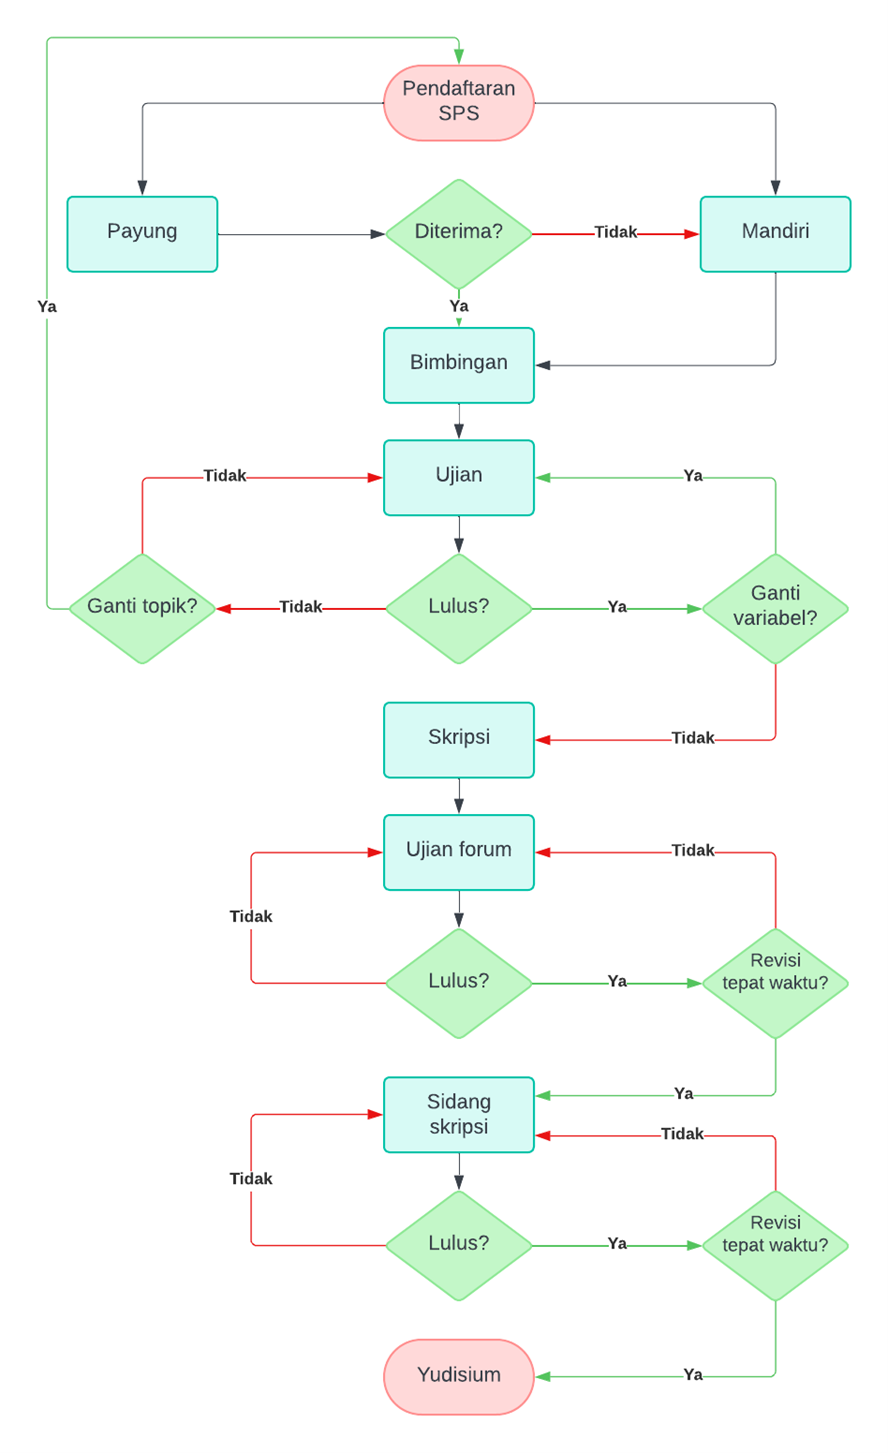
\includegraphics[width=4.6875in,height=\textheight,keepaspectratio]{images/1_1_alurskripsi.png}

}

\caption{Alur Kerja Mata Kuliah Skripsi}

\end{figure}%

\bookmarksetup{startatroot}

\chapter{Memilih Topik Skripsi}\label{memilih-topik-skripsi}

Memilih topik skripsi merupakan langkah pertama dan salah satu yang
paling krusial dalam proses penulisan skripsi. Keputusan ini tidak hanya
akan menentukan arah penelitian Anda selama beberapa bulan atau bahkan
tahun ke depan tetapi juga dapat memengaruhi level motivasi, arah karir,
dan kesuksesan akademis Anda. Oleh karena itu, pemilihan topik yang
tepat dan relevan menjadi sangat penting. Dalam bab ini, kita akan
membahas bagaimana memilih topik yang sesuai, pentingnya relevansi dan
kebaruan topik, serta pentingnya konsultasi dengan pembimbing.

\section{Memahami Minat dan
Kepakaran}\label{memahami-minat-dan-kepakaran}

Langkah pertama dalam memilih topik skripsi adalah introspeksi tentang
apa yang benar-benar Anda minati dan di mana keahlian Anda berada.
Knight dan Steinbach (2008) menyarankan agar mahasiswa memilih topik
yang tidak hanya menarik bagi mereka, tetapi juga sesuai dengan keahlian
dan latar belakang akademis mereka. Hal ini karena penelitian yang
dilakukan dengan minat dan semangat tinggi cenderung menghasilkan karya
yang lebih baik dan proses penelitiannya menjadi lebih menyenangkan.

\section{Relevansi dan Kontribusi terhadap Bidang
Ilmu}\label{relevansi-dan-kontribusi-terhadap-bidang-ilmu}

Selain minat pribadi, relevansi topik terhadap bidang ilmu dan
kemampuannya untuk memberikan kontribusi yang signifikan juga sangat
penting. Menurut Creswell (2014), topik yang dipilih harus mampu mengisi
celah pengetahuan yang ada dalam literatur atau menawarkan perspektif
baru tentang masalah yang sudah ada. Hal ini membutuhkan tinjauan
literatur awal untuk memastikan bahwa penelitian Anda akan memberikan
nilai tambah kepada komunitas ilmiah.

\section{Menentukan Ruang Lingkup
Penelitian}\label{menentukan-ruang-lingkup-penelitian}

Setelah menemukan area minat dan relevansi ilmiah, langkah selanjutnya
adalah menentukan ruang lingkup penelitian Anda. Ruang lingkup yang
terlalu luas dapat membuat penelitian menjadi terlalu kompleks dan sulit
untuk dikelola, sementara ruang lingkup yang terlalu sempit mungkin
tidak cukup menantang atau signifikan. Locke dkk (2010) menyarankan agar
mahasiswa menetapkan batasan yang jelas untuk penelitian mereka,
termasuk aspek temporal, geografis, dan demografis yang akan diteliti.

\section{Konsultasi dengan
Pembimbing}\label{konsultasi-dengan-pembimbing}

Konsultasi dengan dosen pembimbing adalah langkah penting lainnya dalam
proses pemilihan topik. Pembimbing dapat memberikan masukan berharga
tentang kelayakan topik, metodologi yang tepat, dan potensi sumber daya.
Pembimbing juga dapat membantu mengidentifikasi kemungkinan masalah yang
mungkin dihadapi selama penelitian. Bazeley (2013) menekankan pentingnya
membangun hubungan kerja yang baik dengan pembimbing, karena dukungan
dan bimbingannya akan sangat berharga sepanjang proses penelitian.

\section{Memeriksa Ketersediaan Sumber
Daya}\label{memeriksa-ketersediaan-sumber-daya}

Sebelum menetapkan topik skripsi, penting juga untuk mempertimbangkan
ketersediaan sumber daya yang dibutuhkan untuk penelitian. Ini termasuk
akses ke data primer atau sekunder, perangkat lunak analisis data, dan
materi literatur terkait. Ketersediaan sumber daya ini dapat memengaruhi
kelayakan dan keberhasilan penelitian Anda. Kumar (2014) menyarankan
agar mahasiswa melakukan penilaian awal terhadap sumber daya yang
tersedia dan mempertimbangkan alternatif jika sumber daya utama tidak
dapat diakses.

\section*{Kesimpulan}\label{kesimpulan-1}
\addcontentsline{toc}{section}{Kesimpulan}

\markright{Kesimpulan}

Pemilihan topik skripsi adalah proses yang memerlukan pertimbangan
matang dan analisis mendalam. Melalui pemahaman tentang minat pribadi,
relevansi ilmiah, ruang lingkup yang tepat, konsultasi dengan
pembimbing, dan ketersediaan sumber daya, mahasiswa dapat memilih topik
yang tidak hanya memenuhi syarat akademik tetapi juga memuaskan
keingintahuan intelektual mereka. Memilih topik yang tepat adalah
langkah pertama yang penting dalam perjalanan akademis Anda untuk
menyelesaikan skripsi dengan sukses.

\bookmarksetup{startatroot}

\chapter{Struktur Proposal
Penelitian}\label{struktur-proposal-penelitian}

Penyusunan proposal penelitian merupakan fase fundamental dalam
perjalanan akademis setiap mahasiswa. Proposal penelitian berfungsi
sebagai rencana kerja yang menguraikan apa yang akan diteliti, bagaimana
penelitian akan dilakukan, serta mengapa penelitian tersebut penting.
Proposal tidak hanya berfungsi sebagai peta jalan untuk penelitian yang
akan dilakukan tetapi juga sebagai alat untuk meyakinkan pembimbing dan
reviewer tentang nilai dan kelayakan penelitian. Bab ini akan membahas
tentang struktur proposal penelitian yang efektif, pentingnya review
literatur, dan pemilihan metode penelitian yang sesuai.

Proposal penelitian yang baik harus menyajikan informasi yang cukup
untuk meyakinkan pembaca tentang kepentingan dan kelayakan penelitian
yang diusulkan. Struktur proposal umumnya meliputi:

\section{Judul Penelitian}\label{judul-penelitian}

Judul haruslah singkat, informatif, dan menggambarkan esensi dari
penelitian. Sebuah judul yang baik akan langsung memberikan gambaran
tentang topik penelitian serta indikasi metodologi yang digunakan.
Contoh penulisan Judul Penelitian: ``Dampak Media Sosial terhadap
Kesejahteraan Psikologis Remaja''

\section{Bab 1 Pendahuluan}\label{bab-1-pendahuluan}

Bab Pendahuluan dalam sebuah skripsi bertujuan untuk memberikan konteks,
memperkenalkan topik penelitian, dan membangun dasar bagi pembaca
mengenai pentingnya penelitian tersebut. Secara spesifik, tujuan dari
Bab Pendahuluan meliputi:

\begin{enumerate}
\def\labelenumi{\arabic{enumi}.}
\tightlist
\item
  Memperkenalkan topik: Memberikan latar belakang yang memungkinkan
  pembaca memahami topik penelitian dan konteksnya dalam literatur yang
  ada atau masalah praktis yang ditangani.
\item
  Menyatakan masalah penelitian: Mendefinisikan masalah penelitian
  dengan jelas, menunjukkan celah dalam pengetahuan yang ada yang akan
  ditangani oleh penelitian.
\item
  Menyatakan tujuan dan manfaat penelitian: Menguraikan tujuan
  penelitian secara spesifik dan menyajikan manfaat penelitian yang akan
  dihasilkan melalui studi tersebut.
\item
  Menjelaskan signifikansi penelitian: Menggarisbawahi pentingnya
  penelitian ini bagi bidang ilmu pengetahuan, praktik industri, atau
  masyarakat pada umumnya, dan bagaimana penelitian ini akan
  berkontribusi terhadap pengetahuan yang ada.
\item
  Menguraikan ruang lingkup dan batasan: Menjelaskan ruang lingkup
  penelitian dan batasan yang diterapkan untuk memfokuskan studi,
  termasuk apa yang tidak akan ditangani oleh penelitian.
\end{enumerate}

Pada umumnya, struktur penulisan Bab Pendahuluan mencakup empat sub-bab,
yaitu:

\subsection*{Latar Belakang Masalah}\label{latar-belakang-masalah}
\addcontentsline{toc}{subsection}{Latar Belakang Masalah}

Bagian ini merupakan kesempatan untuk ``bercerita'' tentang penelitian
Anda. Sajikan konteks masalah, urgensi penelitiannya, dan bagaimana
penelitian ini dapat memberikan dampak. Gunakan data, statistik, atau
kutipan dari literatur relevan untuk memperkuat argumen Anda tentang
pentingnya masalah penelitian.

Dalam setiap proposal penelitian, latar belakang masalah berfungsi untuk
menggambarkan konteks penelitian, memaparkan masalah yang akan diteliti,
dan menyoroti pentingnya menemukan solusi atau jawaban atas masalah
tersebut. Salah satu aspek kritis dari latar belakang masalah adalah
penjelasan tentang urgensi penelitian. Urgensi ini tidak hanya
menunjukkan kebutuhan untuk menjawab pertanyaan penelitian tetapi juga
mengapa penelitian tersebut penting untuk dilakukan sekarang. Berikut
adalah beberapa aspek yang dapat digunakan untuk menunjukkan urgensi
penelitian:

\begin{enumerate}
\def\labelenumi{\arabic{enumi}.}
\tightlist
\item
  Perkembangan terkini: Adanya perkembangan terkini dalam masyarakat,
  teknologi, atau bidang ilmu pengetahuan yang membutuhkan penelitian
  lebih lanjut. Misalnya, munculnya teknologi baru yang memengaruhi cara
  hidup manusia atau perubahan sosial yang cepat yang belum dipahami
  secara mendalam.
\item
  Gap pengetahuan: Keberadaan gap pengetahuan dalam literatur yang perlu
  diisi. Jika penelitian sebelumnya meninggalkan pertanyaan yang belum
  terjawab atau terdapat kontradiksi antar temuan penelitian, ini
  menciptakan urgensi untuk melakukan penelitian lebih lanjut.
\item
  Masalah sosial yang mendesak: Adanya masalah sosial atau kesehatan
  masyarakat yang mendesak, yang memerlukan solusi berbasis bukti.
  Misalnya, peningkatan kasus penyakit tertentu atau isu-isu lingkungan
  yang memengaruhi kualitas hidup.
\item
  Pengaruh terhadap kebijakan: Urgensi penelitian juga dapat berasal
  dari kebutuhan untuk membentuk atau merevisi kebijakan publik.
  Penelitian yang memberikan bukti baru dapat mendorong pembuatan
  kebijakan yang lebih efektif dan berbasis data.
\item
  Tekanan demografis atau lingkungan: Perubahan demografis, seperti
  penuaan populasi atau migrasi besar-besaran, dan perubahan lingkungan,
  seperti perubahan iklim, yang membutuhkan penelitian untuk memahami
  dampaknya dan mengembangkan strategi adaptasi atau mitigasi.
\end{enumerate}

Dalam menyajikan urgensi penelitian, penting bagi peneliti untuk
menyampaikan bukan hanya mengapa penelitian ini penting secara teoretis,
tetapi juga relevansinya dengan isu-isu praktis, sosial, ekonomi, atau
kebijakan saat ini. Dengan demikian, urgensi penelitian bukan hanya
tentang pentingnya topik itu sendiri tetapi juga tentang waktu dan
konteks di mana penelitian tersebut dilakukan. Menekankan urgensi
penelitian dalam latar belakang masalah tidak hanya menarik minat
pembaca atau penguji, tetapi juga menunjukkan kesadaran peneliti
terhadap dinamika terkini dan pentingnya kontribusi penelitiannya.

\subsection{Rumusan Masalah}\label{rumusan-masalah}

Rumusan masalah harus spesifik, terukur, dan fokus. Ini adalah inti dari
proposal Anda, yang menentukan arah penelitian. Jelaskan secara rinci
pertanyaan penelitian yang ingin Anda jawab dan mengapa pertanyaan ini
penting untuk dikaji lebih lanjut.

\begin{quote}
Contoh penulisan Rumusan Masalah:
\end{quote}

\begin{quote}
Di era digital saat ini, media sosial telah menjadi bagian tak
terpisahkan dari kehidupan sehari-hari, terutama di kalangan remaja.
Meskipun media sosial memberikan manfaat dalam hal konektivitas dan
akses informasi, terdapat kekhawatiran mengenai dampak negatifnya
terhadap kesejahteraan psikologis remaja, termasuk peningkatan
kecemasan, depresi, dan gangguan citra tubuh. Namun, penelitian yang
mengkaji secara mendalam hubungan antara penggunaan media sosial dan
kesejahteraan psikologis remaja masih terbatas. Oleh karena itu, perlu
dilakukan studi lebih lanjut untuk mengidentifikasi sejauh mana
penggunaan media sosial mempengaruhi kesejahteraan psikologis remaja dan
faktor-faktor yang memoderasi dampak tersebut.
\end{quote}

\subsection{Tujuan Penelitian}\label{tujuan-penelitian}

Sajikan tujuan penelitian Anda secara jelas dan langsung. Tujuan harus
selaras dengan rumusan masalah dan memberikan gambaran tentang apa yang
ingin dicapai melalui penelitian.

\begin{quote}
Contoh penulisan Tujuan Penelitian:

Tujuan utama dari penelitian ini adalah untuk menginvestigasi dampak
penggunaan media sosial terhadap kesejahteraan psikologis remaja. Secara
khusus, penelitian ini bertujuan untuk:

\begin{enumerate}
\def\labelenumi{\arabic{enumi}.}
\tightlist
\item
  Mengukur tingkat penggunaan media sosial di kalangan remaja.
\item
  Menilai kesejahteraan psikologis remaja dengan menggunakan skala
  kesejahteraan psikologis yang valid dan reliabel.
\item
  Menentukan hubungan antara penggunaan media sosial dan kesejahteraan
  psikologis remaja.
\item
  Mengidentifikasi faktor-faktor yang memoderasi hubungan antara
  penggunaan media sosial dan kesejahteraan psikologis, seperti dukungan
  sosial, jenis kelamin, dan aktivitas fisik.
\end{enumerate}
\end{quote}

\subsection{Manfaat Penelitian}\label{manfaat-penelitian}

Di bagian ini, gambarkan kontribusi penelitian Anda terhadap ilmu
pengetahuan, praktik industri dan kebijakan, atau masyarakat umum. Ini
adalah kesempatan untuk meyakinkan pembaca tentang nilai tambah dari
penelitian Anda.

\begin{quote}
Contoh penulisan Manfaat Penelitian:

Penelitian ini diharapkan dapat memberikan manfaat sebagai berikut:

\begin{enumerate}
\def\labelenumi{\arabic{enumi}.}
\tightlist
\item
  Teoretis: Memberikan kontribusi pada literatur psikologi dengan
  memperdalam pemahaman mengenai hubungan antara penggunaan media sosial
  dan kesejahteraan psikologis remaja. Penelitian ini juga dapat
  menawarkan wawasan tentang mekanisme yang mendasari hubungan tersebut
  dan faktor-faktor yang memengaruhi dampak media sosial.
\item
  Praktis untuk individu: Memberikan informasi kepada remaja dan orang
  tua tentang potensi dampak negatif dan positif dari penggunaan media
  sosial terhadap kesejahteraan psikologis, sehingga mereka dapat
  membuat keputusan yang lebih terinformasi tentang penggunaan media
  sosial.
\item
  Praktis untuk pembuat kebijakan: Hasil penelitian ini dapat dijadikan
  dasar oleh pembuat kebijakan dan praktisi pendidikan dalam
  mengembangkan program dan intervensi untuk mengurangi dampak negatif
  media sosial pada remaja, serta memanfaatkan potensi positifnya untuk
  mendukung kesejahteraan psikologis.
\item
  Sosial: Meningkatkan kesadaran masyarakat tentang pentingnya
  penggunaan media sosial yang sehat di kalangan remaja dan dampaknya
  terhadap kesehatan mental.
\end{enumerate}
\end{quote}

\section{Bab 2 Tinjauan Literatur}\label{bab-2-tinjauan-literatur}

Tinjauan literatur dalam proposal penelitian bukan hanya sekadar daftar
pustaka yang telah dibaca. Menurut Creswell (2014), tinjauan literatur
harus menunjukkan pemahaman mendalam tentang masalah yang diteliti,
mengidentifikasi gap dalam literatur, dan mendukung kebutuhan untuk
penelitian Anda. Proses ini memungkinkan peneliti untuk memposisikan
penelitiannya dalam konteks penelitian terdahulu, serta membangun dasar
teori yang kokoh untuk penelitian.

Secara umum, Bab Tinjauan Literatur mencakup pembahasan mengenai:

\begin{enumerate}
\def\labelenumi{\arabic{enumi}.}
\tightlist
\item
  Variabel penelitian: Bagian ini berisi penjelasan mengenai variabel
  utama dalam penelitian, termasuk variabel independen, dependen, dan
  moderating/mediating jika ada.
\item
  Definisi variabel/konstruk: Berisi penjelasan secara ringkas dan padat
  mengenai definisi konseptual variabel atau konstruk psikologis yang
  diteliti. Peneliti perlu menuliskan definisi dari konsep-konsep kunci
  yang akan digunakan dalam penelitian. Selain itu, peneliti juga
  menjelaskan bagaimana konsep ini diukur atau didefinisikan dalam
  konteks penelitian, jika menggunakan metode pengukuran khusus.
\item
  Teori utama: Uraian teori-teori kunci yang membentuk dasar konseptual
  untuk penelitian. Di bagian ini, peneliti perlu menjelaskan sejarah,
  pengembangan, dan aplikasi teori dalam penelitian sebelumnya.
\item
  Temuan studi sebelumnya: Bagian ini berisi tinjauan
  penelitian-penelitian penting yang telah dilakukan terkait dengan
  topik penelitian. Secara lebih lanjut, peneliti membahas tentang
  metodologi, temuan, dan kontribusi mereka terhadap bidang studi.
\item
  Studi terkait lainnya: Peneliti diharapkan mampu menjelaskan studi
  atau eksperimen terkait lainnya yang mungkin tidak langsung terkait
  dengan pertanyaan penelitian tetapi memberikan konteks atau pendukung
  teoretis yang relevan.
\item
  Dinamika antar variabel: Analisis dan sintesis temuan dari seluruh
  literatur dan studi yang telah ditinjau tersebut untuk menunjukkan
  bagaimana mereka berkontribusi pada pemahaman saat ini tentang topik
  dan mengidentifikasi celah dalam literatur. Untuk penelitian dengan
  metode kuantitatif, bagian ini diakhiri dengan pernyataan rumusan
  hipotesis penelitian. Rumusan hipotesis yang dituliskan harus
  berkesuaian dengan penjelasan penjelasan mengenai kaitan antar
  variabel yang telah dibahas. Misalnya: ``Berdasarkan uraian mengenai
  stres kerja dan burnout yang telah disampaikan, penulis berhipotesis
  bahwa stres kerja berkorelasi positif dengan persepsi mengenai burnout
  pada pekerja di bidang kesehatan.''
\end{enumerate}

\section{Bab 3 Metode Penelitian
Penulisan}\label{bab-3-metode-penelitian-penulisan}

Bab Metode Penelitian dalam skripsi dirancang untuk memberikan pembaca
pemahaman yang jelas tentang bagaimana penelitian dilakukan. Bab ini
menjelaskan dengan rinci desain penelitian, pendekatan metodologis,
prosedur pengumpulan data, instrumen yang digunakan, serta teknik
analisis data. Berikut adalah struktur penulisan Bab 3 Metode
Penelitian:

\subsection{Pendekatan, rancangan, dan jenis
penelitian}\label{pendekatan-rancangan-dan-jenis-penelitian}

Di bagian awal Bab Metode ini peneliti menjelaskan apakah penelitian
bersifat kuantitatif, kualitatif, atau mixed methods, serta alasan
pemilihan jenis penelitian tersebut. Peneliti harus dapat menguraikan
justifikasi untuk desain penelitian yang dipilih, termasuk bagaimana
desain ini akan membantu menjawab pertanyaan penelitian atau menguji
hipotesis.

\subsection{Populasi dan sampel (riset
kuantitatif)}\label{populasi-dan-sampel-riset-kuantitatif}

Deskripsikan populasi target untuk penelitian Anda dan alasan pemilihan
populasi ini. Gambarkan secara detil kriteria atau karakteristik sampel
yang dilibatkan dalam penelitian. Jelaskan teknik sampling yang
digunakan (misalnya, random sampling, purposive sampling) dan proses
untuk memilih sampel dari populasi. Sertakan ukuran sampel dan
justifikasi untuk ukuran ini berdasarkan pertimbangan statistik atau
metodologis.

\subsection{Situs/kasus dan partisipan/informan (riset
kualitatif)}\label{situskasus-dan-partisipaninforman-riset-kualitatif}

Dalam penelitian kualitatif, istilah ``populasi'' sering digantikan
dengan ``kasus'' atau ``situs penelitian''. Kasus ini bisa berupa
individu, grup, organisasi, komunitas, atau bahkan suatu peristiwa.
Dalam proses pengumpulan data, penelitian kualitatif berfokus pada
``partisipan'' atau ``informan'' yang dipilih untuk studi. Partisipan
ini dipilih karena mereka dianggap memiliki pengalaman, pengetahuan,
atau wawasan yang mendalam tentang topik penelitian. Beberapa strategi
pemilihan partisipan yang umum dalam penelitian kualitatif meliputi
purposive sampling, extreme or deviant case sampling, snowball sampling,
dan theoretical sampling.

\subsection{Variabel penelitian/Gejala
penelitian/Fenomena}\label{variabel-penelitiangejala-penelitianfenomena}

Bagian ini menguraikan dan mendefinisikan variabel yang akan diteliti,
termasuk variabel independen, dependen, mediasi, moderasi, dan kontrol
jika ada. Dalam uraiannya, peneliti menjelaskan definisi konseptual dan
definisi operasional dari variabel tersebut. Definisi konseptual
berfokus pada penjelasan teoretis dan makna konseptual variabel,
sedangkan definisi operasional berfokus pada pengukuran praktis dan cara
variabel dioperasionalkan dalam penelitian. Misalnya, dalam sebuah
penelitian mengenai stres, maka penulis dapat menjelaskan bahwa secara
konsptual, stres didefinisikan sebagai ``suatu kondisi psikologis yang
dialami individu ketika ia merasakan tuntutan yang melebihi sumber daya
pribadi dan sosial yang mereka miliki untuk mengatasinya.'' Lebih
lanjut, secara operasional, stres didefinisikan sebagai ``skor yang
diperoleh dari jawaban kuesioner Perceived Stress Scale (PSS-10), di
mana skor yang lebih tinggi menunjukkan tingkat stres yang lebih
tinggi.''

\subsection{Hipotesis}\label{hipotesis}

Jika penelitian Anda kuantitatif, formulasikan hipotesis yang akan diuji
berdasarkan kerangka teoretis dan kajian literatur yang telah diuraikan.
Peneliti tidak perlu menuliskan hipotesis nol di bagian ini karena bukan
merupakan hipotesis yang diajukan oleh peneliti. Hipotesis
diformulasikan sespesifik mungkin, relevan dengan variabel dan populasi
penelitian, serta tidak ditulis dalam bentuk hipotesis umum. Perumusan
hipotesis juga harus menggunakan definisi operasional dari variabel yang
diteliti. Contoh penulisan hipotesis penelitian: ``Kualitas tidur yang
lebih baik berkorelasi dengan kinerja akademik yang lebih tinggi di
kalangan mahasiswa semester akhir. Dalam hal ini, mahasiswa yang
melaporkan skor Quality of Sleep Scale yang tinggi cenderung memperoleh
nilai IPK yang tinggi juga, begitu pula sebaliknya.''

Dalam riset kualitatif, peneliti tidak perlu menuliskan hipotesis
penelitian karena pada prinsipnya penelitian kualitatif berfokus pada
pemahaman mendalam tentang pengalaman, persepsi, dan konstruksi sosial
individu atau kelompok. Tujuannya adalah untuk mengeksplorasi dan
menginterpretasi makna dibandingkan untuk mengukur variabel atau menguji
hipotesis secara statistik.

\subsection{Instrumen penelitian}\label{instrumen-penelitian}

Jelaskan instrumen yang digunakan untuk mengumpulkan data, seperti
kuesioner, wawancara, observasi, atau instrumen lainnya. Pada penelitian
kuantitatif, bagian ini juga memuat informasi detil mengenai properti
psikometris alat ukur yang digunakan, mencakup reliabilitas, validitas,
dan norma (jika ada) alat ukur. Penjelasan mengenai properti psikometris
ini dapat dimulai dengan penyampaian kesimpulan hasil uji psikometris
pada penelitian-penelitian sebelumnya.

Informasi mengenai hasil adaptasi alat ukur di berbagai budaya dapat
memperkaya pemahaman pembaca mengenai kualitas psikometris alat ukur.
Peneliti juga perlu menjelaskan proses adaptasi yang akan dilakukan jika
menggunakan alat ukur yang belum pernah diadaptasi ke budaya Indonesia
sebelumnya. Jika alat ukur pernah diadaptasi dalam penelitian lain,
peneliti hanya cukup mengutip informasi dari hasil pengujian adaptasi
yang telah dilakukan. Terakhir, laporkan rencana proses pengujian
reliabilitas dan analisis item alat ukur yang dilakukan melalui uji
coba, serta modifikasi yang dilakukan berdasarkan hasil pengujian
tersebut.

Pada penelitian kualitatif, laporan mengenai reliabilitas berkaitan
dengan transparansi dan konsistensi dalam pengumpulan dan analisis data.
Peneliti perlu menjabarkan strategi yang akan dilakukan untuk
menunjukkan bahwa interpretasi data dilakukan dengan cara-cara yang
dapat dipertanggungjawabkan, misalnya melalui audit data atau
pemeriksaan konsistensi kode data. Validitas dalam penelitian kualitatif
berkaitan dengan keakuratan dan relevansi interpretasi peneliti terhadap
data, sering disebut sebagai kredibilitas, transferabilitas,
dependabilitas, dan konfirmabilitas. Sejumlah strategi dapat dilakukan,
seperti triangulasi, member checking, dan thick description.

\subsection{Prosedur}\label{prosedur}

Peneliti harus dapat menjelaskan secara detil prosedur pengumpulan data,
termasuk langkah-langkah yang diambil, waktu dan tempat pengumpulan
data, dan cara data direkam atau didokumentasikan. Hal ini dilakukan
untuk memenuhi prinsip replikabilitas sebuah karya ilmiah. Artinya,
peneliti harus dapat mendeskripsikan prosedur penelitian dengan sangat
baik sehingga peneliti lain dapat melakukan penelitian serupa dengan
prosedur yang sama demi kepentingan replikasi penelitian. Penting bagi
peneliti untuk menjelaskan prosedur penelitian secara kronologis.
Peneliti juga perlu menjelaskan media yang digunakan dalam proses
pengumpulan data, misalnya dengan menggunakan platform online. Jika
perlu, peneliti dapat menampilkan diagram prosedur untuk membantu
pembaca memahami seluruh langkah dan tahapan pengumpulan data.

\subsection{Metode analisis data}\label{metode-analisis-data}

Pada bagian ini, peneliti menuliskan rencana metode yang dipilih untuk
menganilisis data yang akan dikumpulkan. Pemilihan metode ini harus
disesuaikan dengan jenis datanya, serta kesesuaian dengan pertanyaan
penelitian atau hipotesis yang telah dirumuskan. Selain itu, peneliti
juga menjelaskan alat bantu yang digunakan dalam melakukan analisis
data, misalnya, perangkat lunak. Pada metode kuantitatif, metode
analisis dapat mencakup dari analisis deskriptif, seperti rata-rata dan
deviasi standar, hingga analisis inferensial, seperti korelasi, regresi,
uji-t, dan ANOVA. Sedangkan, pada metode kualitatif, analisis data dapat
dilakukan dengan coding, analisis tematik, dan analisis naratif.

\section{Daftar Pustaka}\label{daftar-pustaka}

Daftar pustaka harus mencakup semua sumber yang telah Anda kutip dalam
proposal. Gunakan gaya sitasi APA terkini yang konsisten dan pastikan
semua sumber terdaftar dengan benar. Anda diwajibkan menggunakan
reference manager (seperti: Mendeley, EndNote, Zetero, dsb) dalam
menuliskan kutipan dan daftar pustaka. Penjelasan lebih lengkap mengenai
format penulisan beserta contoh penulisan Daftar Pustaka akan
disampaikan dalam bagian tersendiri di Bab 6.

\section*{Kesimpulan}\label{kesimpulan-2}
\addcontentsline{toc}{section}{Kesimpulan}

\markright{Kesimpulan}

Penyusunan proposal penelitian yang efektif adalah langkah awal yang
penting dalam proses penulisan skripsi. Proposal yang baik tidak hanya
menyajikan rencana kerja yang logis dan terorganisir, tetapi juga
menunjukkan pentingnya dan relevansi penelitian yang diusulkan.


\backmatter


\end{document}
